\chapter{Imagens}
\label{chap:appendix}

\section{Visualizações específicas}

\begin{figure}[H]
    \centering
    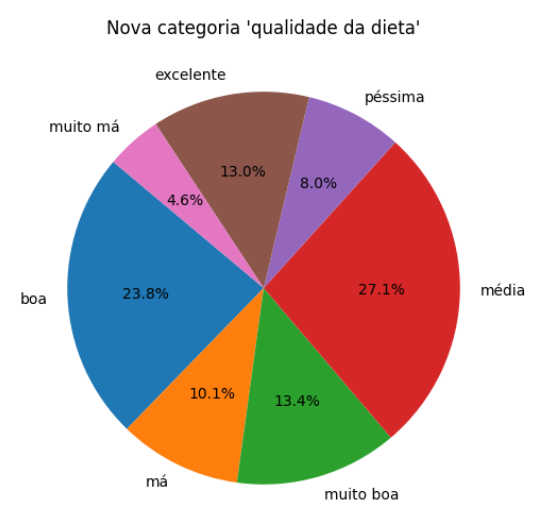
\includegraphics[scale=0.5]{images/dieta.png}
    \caption{Nova categoria 'qualidade da dieta' feita através das categorias de consumo.}
    \label{fig:dieta}
\end{figure}

\begin{figure}[H]
    \centering
    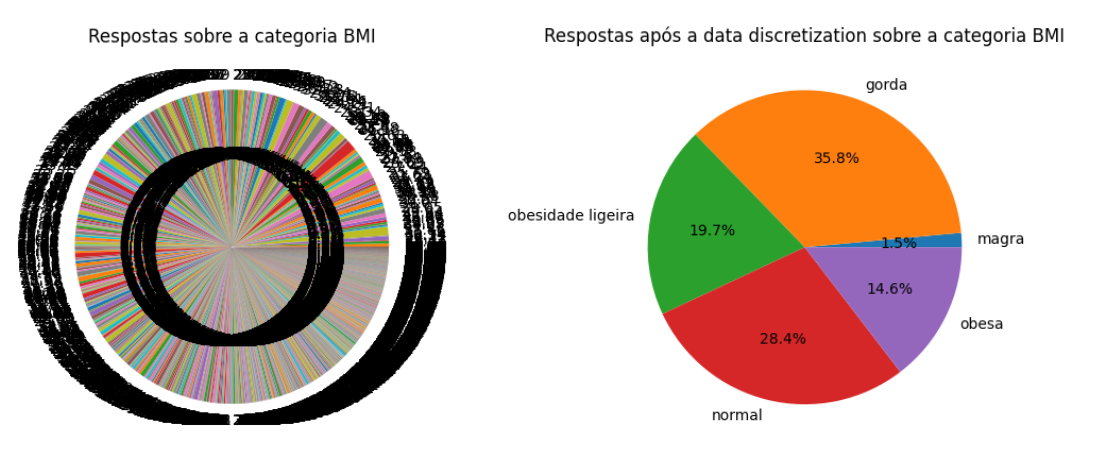
\includegraphics[scale=0.45]{images/BMI.png}
    \caption{Valores da categoria 'BMI' antes e depois da aplicação da discretização dos dados.}
    \label{fig:bmi}
\end{figure}

\begin{figure}[H]
    \centering
    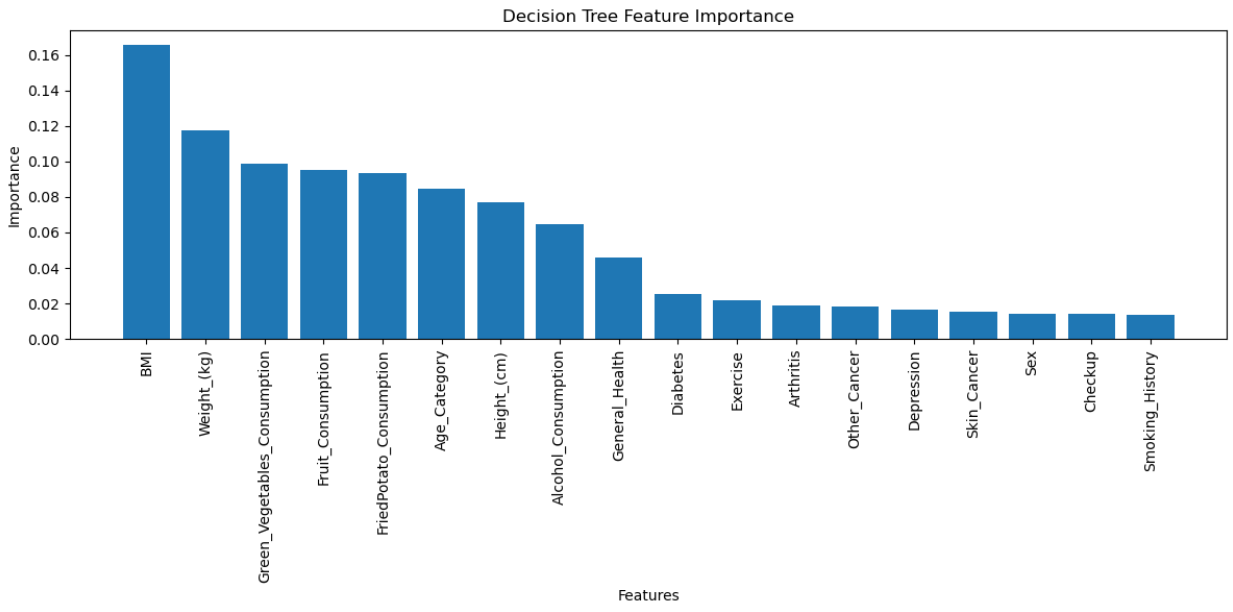
\includegraphics[width=0.9\textwidth]{images/feature_importance.png}
    \caption{\textit{Decision Trees}: Importância das variáveis identificadas pelo modelo.}
    \label{fig:feature_importance}
\end{figure}

\begin{figure}[H]
    \centering
    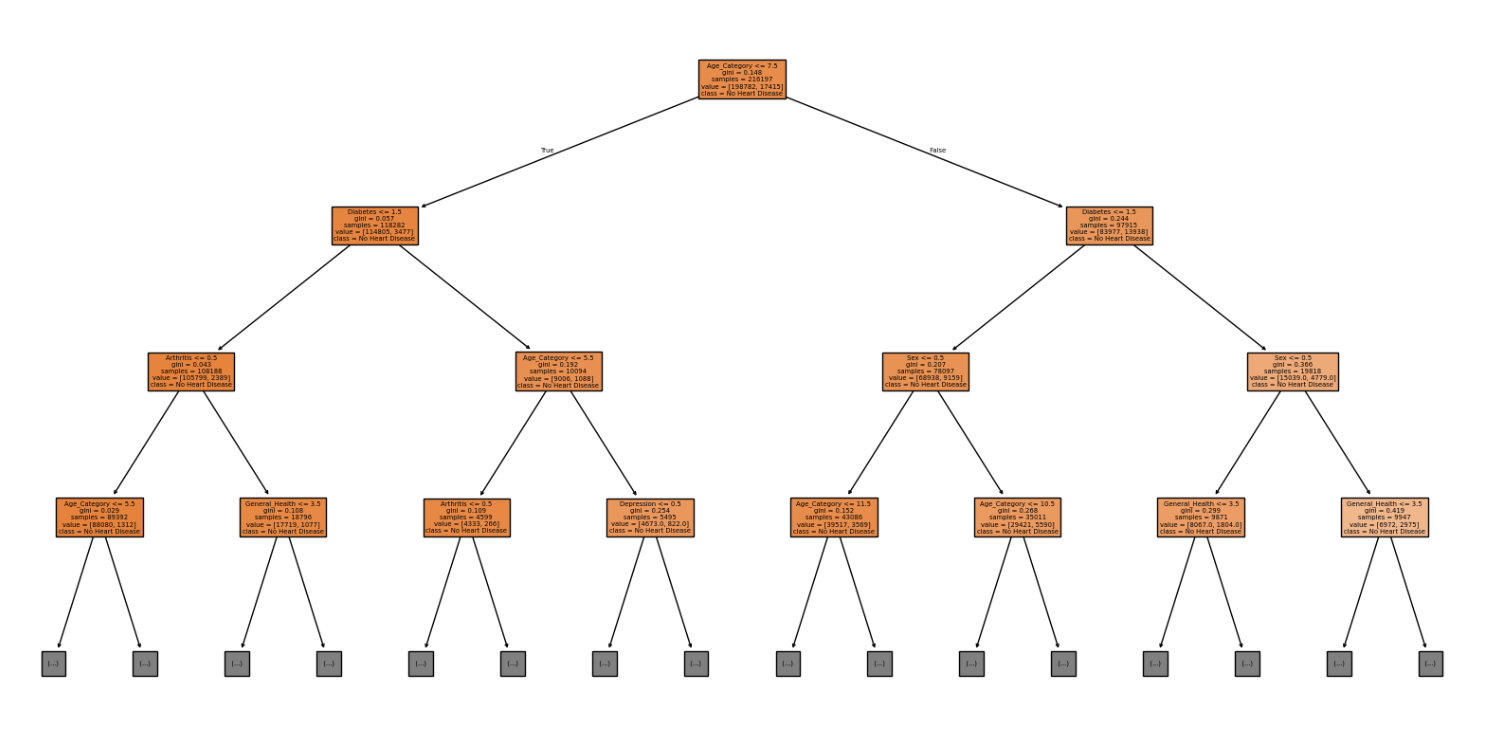
\includegraphics[width=0.9\textwidth]{images/decision_tree_structure.png}
    \caption{\textit{Decision Trees}: Visualização detalhada da estrutura da árvore gerada pelo modelo.}
    \label{fig:decision_tree_structure}
\end{figure}

\begin{figure}[H]
    \centering
    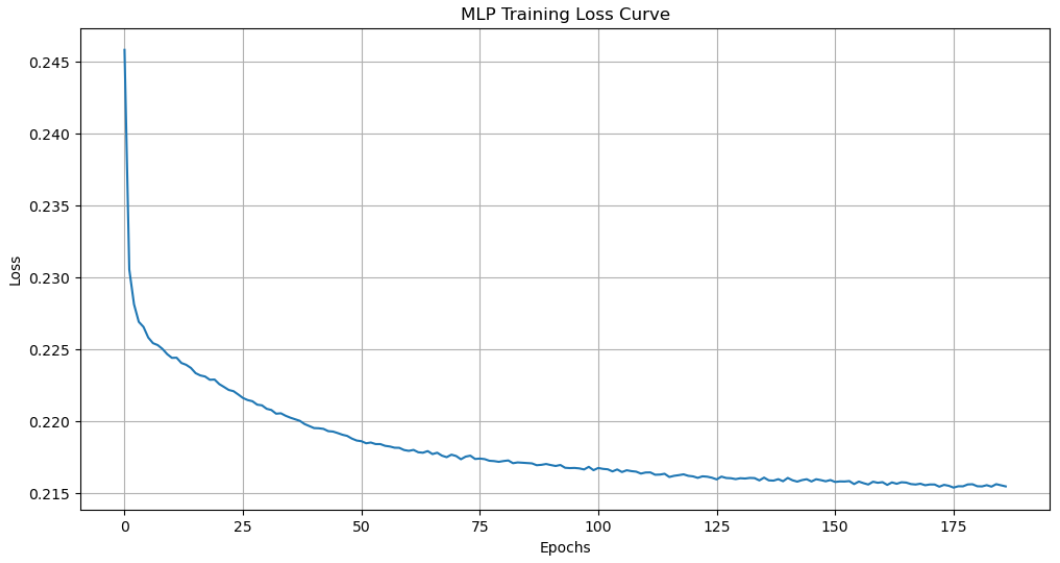
\includegraphics[width=0.9\textwidth]{images/mlp_training_loss.png}
    \caption{\textit{Multi-layer Perceptron}: Curva de perda durante o treino, mostrando a convergência do modelo.}
    \label{fig:mlp_training_loss}
\end{figure}

\begin{figure}[H]
    \centering
    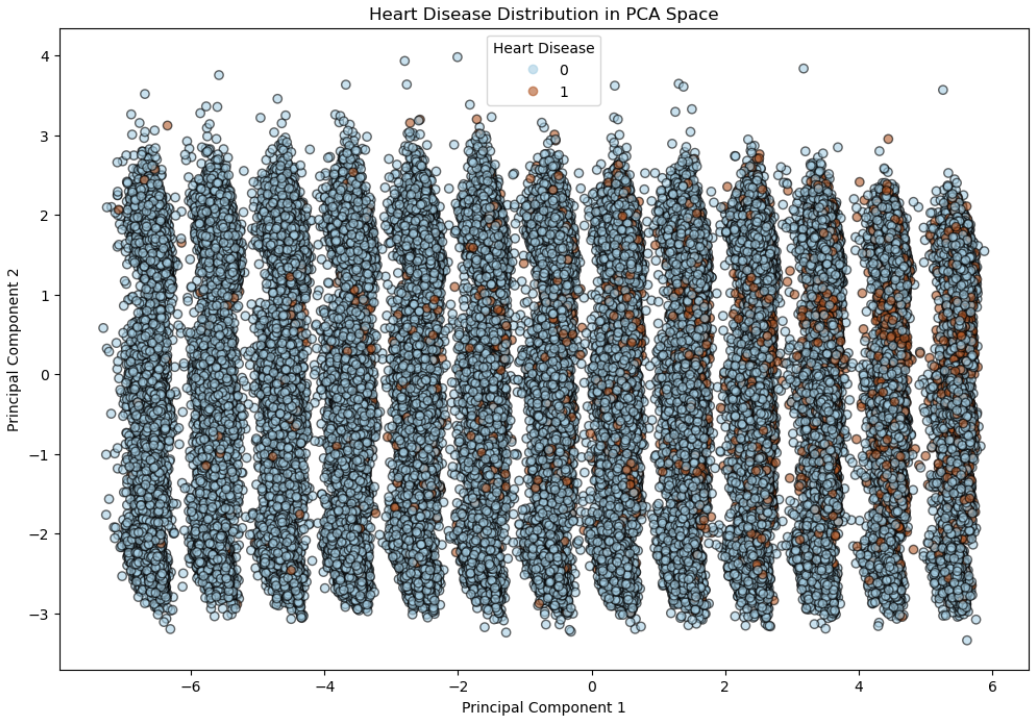
\includegraphics[width=0.9\textwidth]{images/knn_pca.png}
    \caption{\textit{k-NN}: Distribuição dos dados no espaço reduzido para 2 dimensões utilizando \textit{PCA}.}
    \label{fig:knn_pca}
\end{figure}

\section{Métricas individuais de modelos}
\begin{figure}[H]
    \centering
    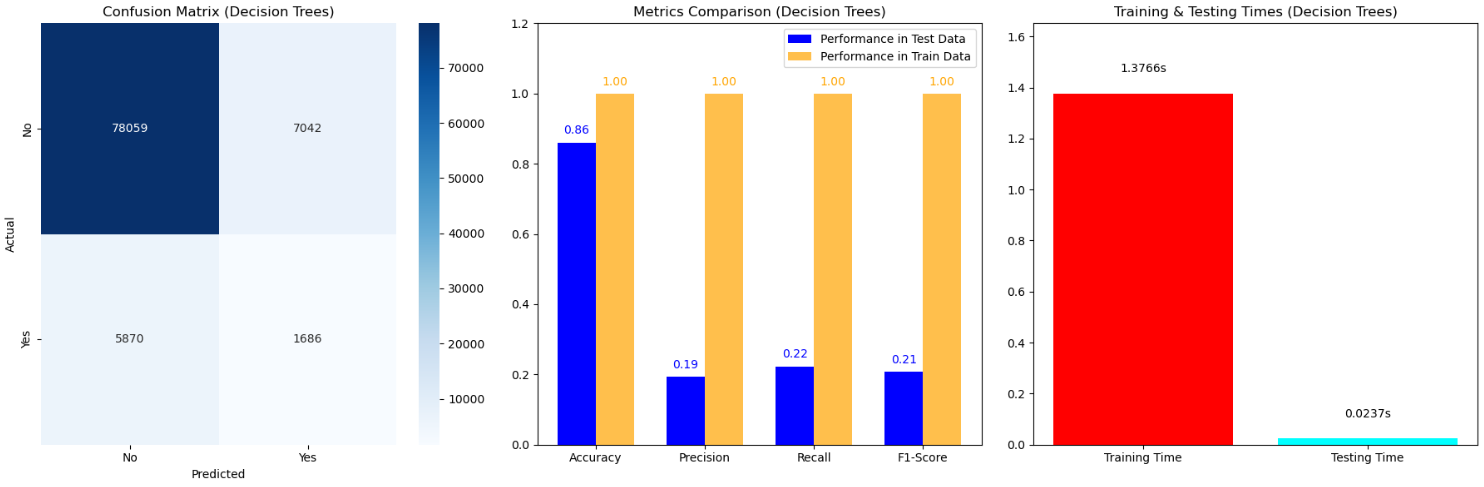
\includegraphics[width=0.9\textwidth]{images/decision_tree_overview.png}
    \caption{Modelo de \textit{Decision Trees}: Matriz de confusão, métricas de desempenho e tempos de execução.}
    \label{fig:decision_tree_overview}
\end{figure}

\begin{figure}[H]
    \centering
    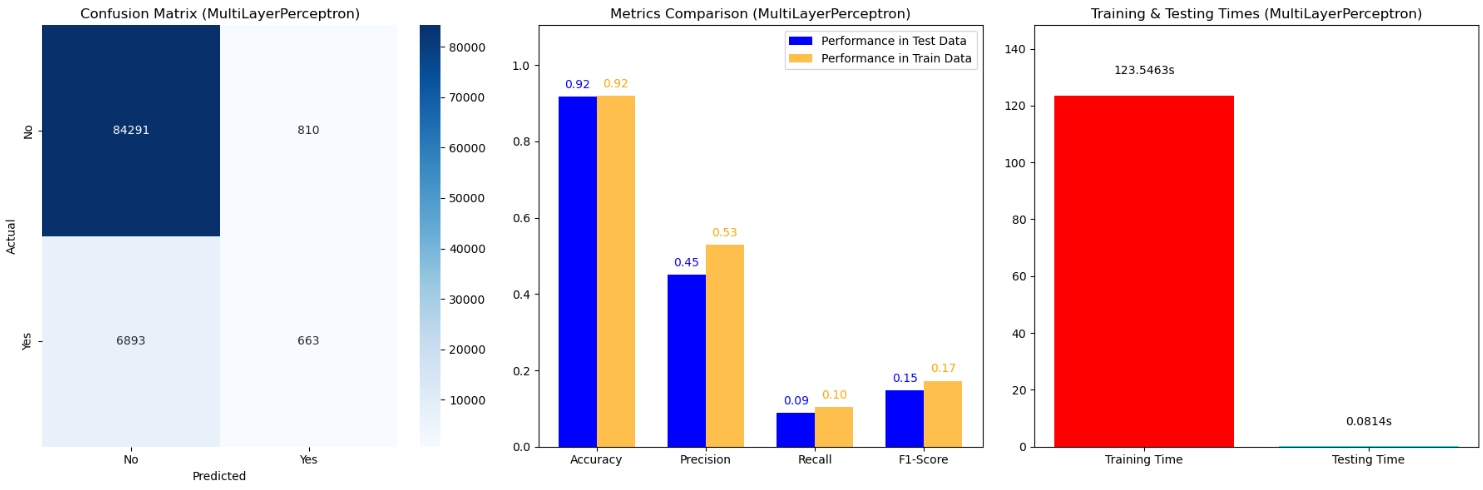
\includegraphics[width=0.9\textwidth]{images/mlp_overview.png}
    \caption{Modelo de \textit{Multi-layer Perceptron}: Matriz de confusão, métricas de desempenho e tempos de execução.}
    \label{fig:mlp_overview}
\end{figure}

\begin{figure}[H]
    \centering
    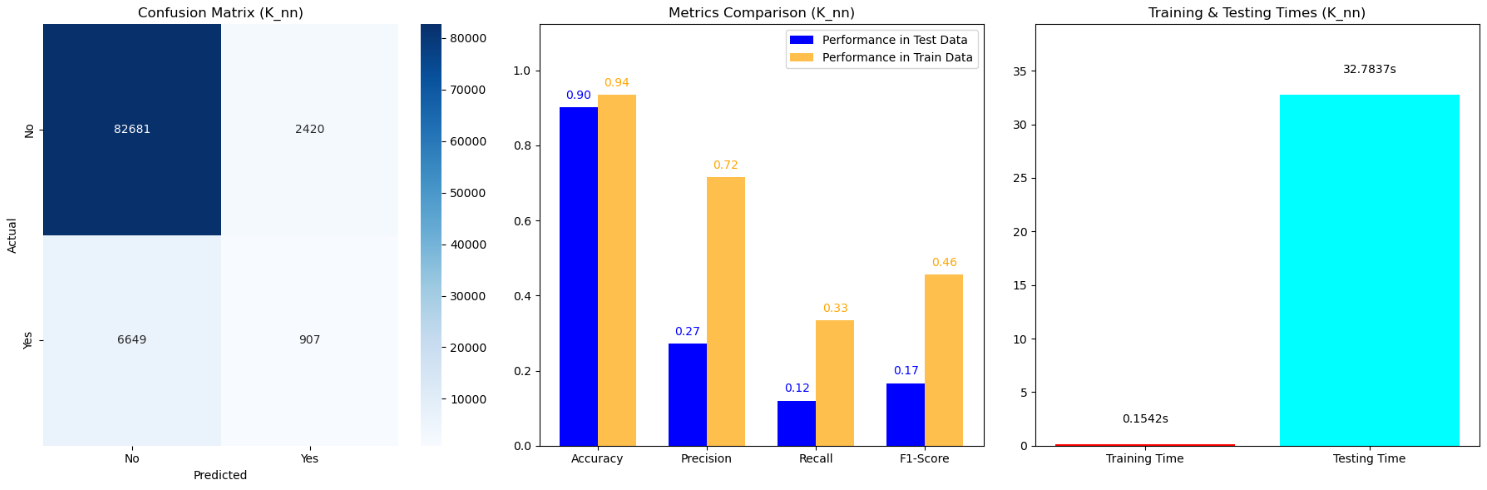
\includegraphics[width=0.9\textwidth]{images/knn_overview.png}
    \caption{Modelo de \textit{k-NN}: Matriz de confusão, métricas de desempenho e tempos de execução.}
    \label{fig:knn_overview}
\end{figure}

\section{Comparações}
\label{chap:comparacoes}

\begin{figure}[H]
    \centering
    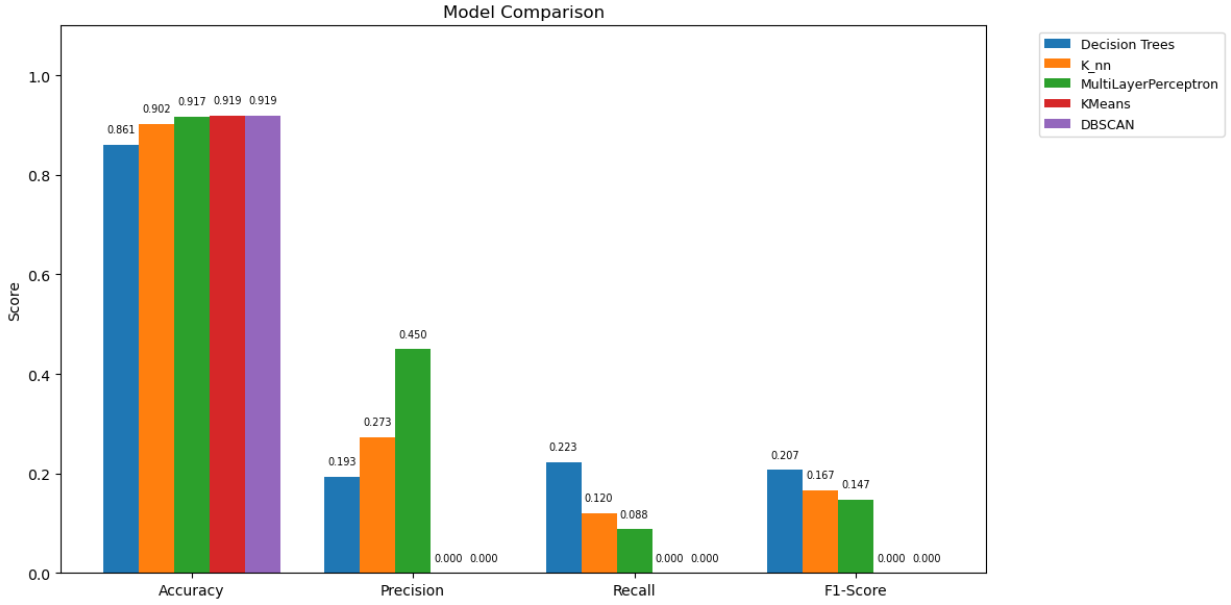
\includegraphics[width=0.9\textwidth]{images/model_comparison.png}
    \caption{Comparação geral do desempenho de todos os modelos.}
    \label{fig:model_comparison}
\end{figure}

\begin{figure}[H]
    \centering
    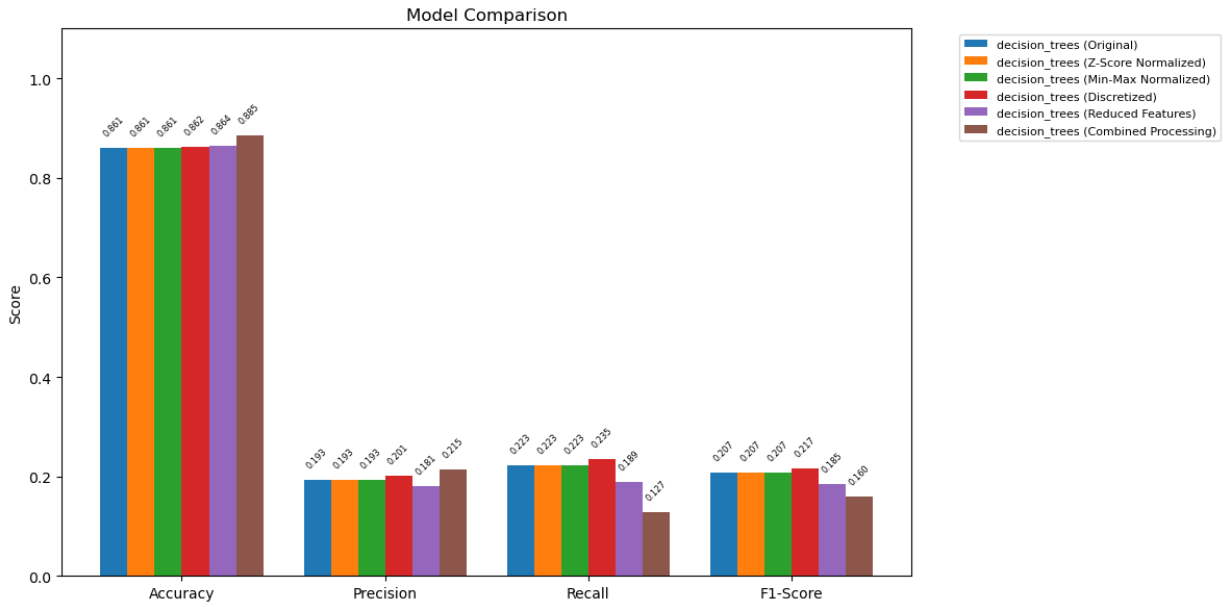
\includegraphics[width=0.9\textwidth]{images/decision_trees_comparison.png}
    \caption{\textit{Decision Trees}: Impacto de diferentes preparações dos dados no desempenho do modelo.}
    \label{fig:decision_trees_comparison}
\end{figure}

\begin{figure}[H]
    \centering
    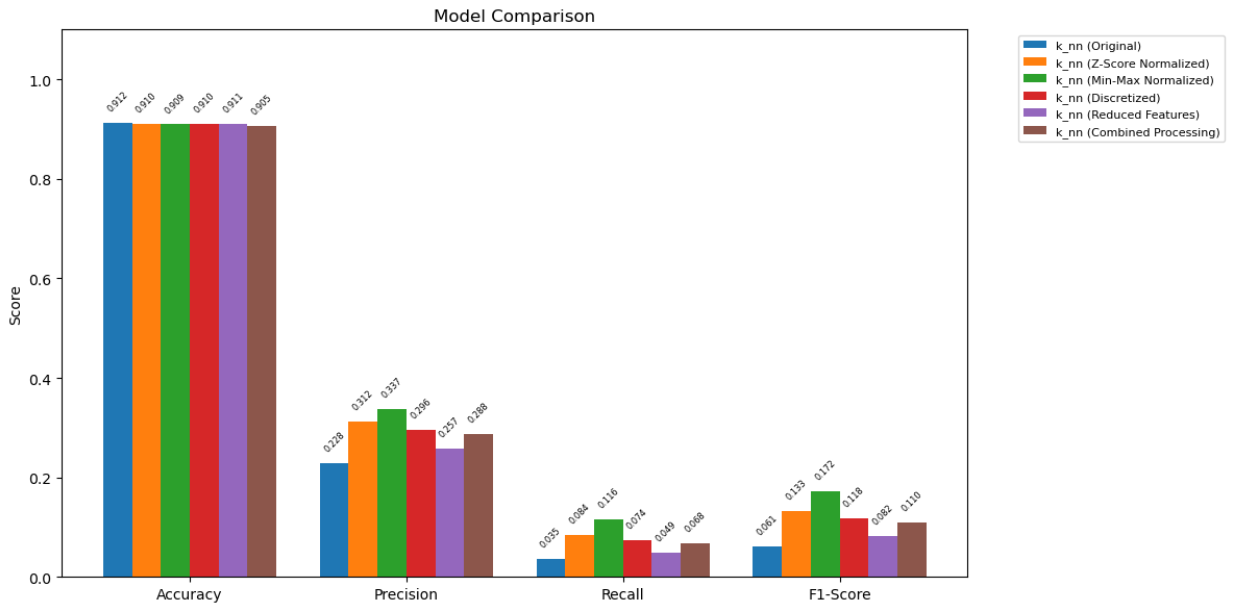
\includegraphics[width=0.9\textwidth]{images/knn_comparison.png}
    \caption{\textit{k-NN}: Impacto de diferentes preparações dos dados no desempenho do modelo.}
    \label{fig:knn_comparison}
\end{figure}

\begin{figure}[H]
    \centering
    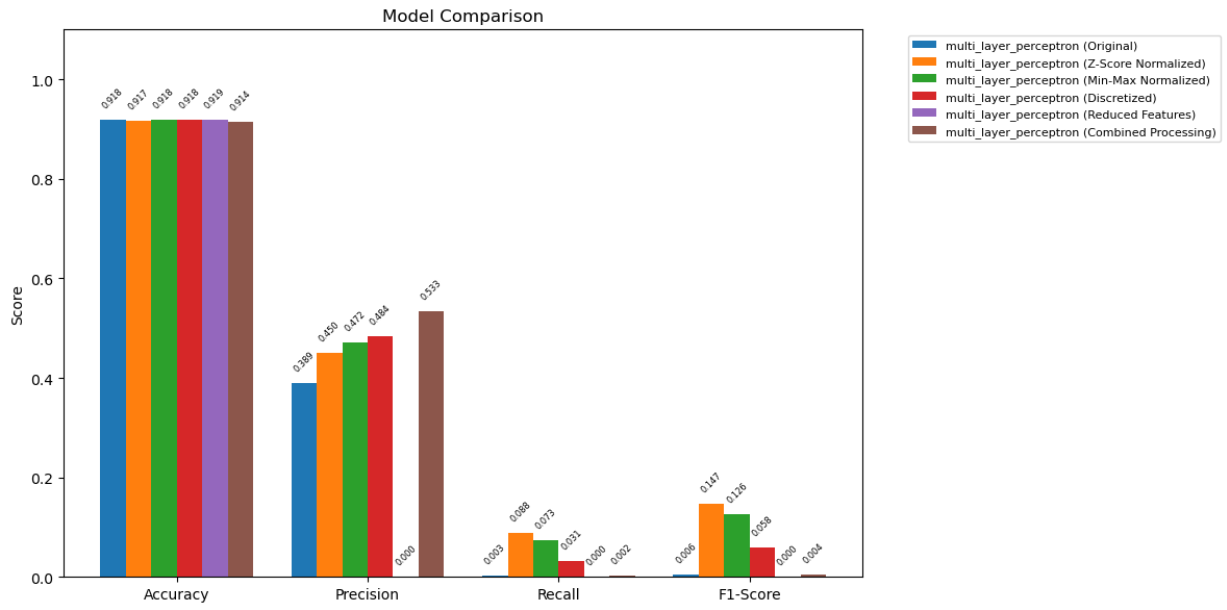
\includegraphics[width=0.9\textwidth]{images/mlp_comparison.png}
    \caption{\textit{Multi-layer Perceptron}: Impacto de diferentes preparações dos dados no desempenho do modelo.}
    \label{fig:mlp_comparison}
\end{figure}


\begin{lstlisting}[caption={Excerto de código utilizado para calcular o valor da dieta a partir das categorias de consumo}, language=Python, label={codigo:dieta}]
# calculo para obter o valor da dieta da pessoa:
# valor_da_dieta = fruta + vegetais - alcool*4 - batata
numeros = dataset.iloc[:, 14] + dataset.iloc[:, 15] - dataset.iloc[:, 13]*4 - dataset.iloc[:, 16]

# calcular a media e o desvio
media = np.mean(numeros)
desvio = np.std(numeros)*0.5

# calcular os valores para as condicoes de cada label, usando a media e um desvio
valores_correspondentes = [media - 3 * desvio, media - 2 * desvio, media - desvio, media, media + desvio, media + 2 * desvio, media + 3 * desvio]
\end{lstlisting}

\begin{lstlisting}[caption={Excerto de código utilizado para substituir todos os valores numericos da categoria 'Height (cm)' por valores categoricos.}, language=Python, label={codigo:data_disc}]
# ALTURA -> em vez de usar os valores verdadeiros da altura, reduzir para algumas categorias genericas
for i in range(len(dataset[11])):
    if dataset[11][i] < 150: # +1.5m
			dataset[11][i] = "<150"
    elif dataset[11][i] >= 150 and dataset[11][i] <=160: # entre 1.5 e 1.6 m
			dataset[11][i] = "150-160"
    elif dataset[11][i] > 160 and dataset[11][i] <=170: # entre 1.6 e 1.7 m
			dataset[11][i] = "161-170"
    elif dataset[11][i] > 170 and dataset[11][i] <=180: # entre 1.7 e 1.8 m
			dataset[11][i] = "171-180"
    elif dataset[11][i] > 180 and dataset[11][i] <=190: # entre 1.8 e 1.9 m
			dataset[11][i] = "181-190"
    elif dataset[11][i] > 190 and dataset[11][i] <=200: # entre 1.9 e 2.0 m
			dataset[11][i] = "191-200"
    else: # +2.0m
			dataset[11][i] = ">200"
\end{lstlisting}